\documentclass[tikz,border=2mm]{standalone}
\usepackage{graphicx}
\usepackage{amsmath}
\usepackage{helvet}
\renewcommand{\familydefault}{\sfdefault}
\usetikzlibrary{arrows.meta,positioning,fit,calc,shapes.geometric,backgrounds}

\definecolor{ink}{HTML}{1F2937}
\definecolor{muted}{HTML}{64748B}
\definecolor{panel}{HTML}{F8FAFC}
\definecolor{edge}{HTML}{CBD5E1}
\definecolor{tiny}{HTML}{E69F00}
\definecolor{small}{HTML}{56B4E9}
\definecolor{medium}{HTML}{009E73}
\definecolor{large}{HTML}{0072B2}
\definecolor{risk}{HTML}{CC79A7}
\definecolor{hardware}{HTML}{475569}

\tikzset{
  arr/.style={-{Latex[length=1.8mm,width=1.3mm]}, line width=0.65pt, draw=ink},
  card/.style={draw=edge, rounded corners=1.5mm, fill=white, line width=0.7pt,
               inner sep=1.4mm, align=center, font=\sffamily},
  stage/.style={card, minimum height=18mm},
  smalltext/.style={font=\sffamily\fontsize{6.4}{7.2}\selectfont, text=muted},
  title/.style={font=\sffamily\fontsize{7.3}{8.2}\selectfont\bfseries, text=ink},
}

\begin{document}
\begin{tikzpicture}[x=1mm,y=1mm]
  \node[card, anchor=south west, inner sep=0.8mm] (input) at (0,19)
    {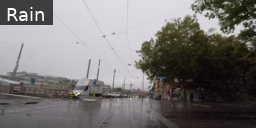
\includegraphics[width=20mm,height=10mm]{assets/fig3_input.png}};
  \node[title, anchor=south] at ([yshift=1.8mm]input.north) {Adverse image};

  \node[card, anchor=south west, inner sep=0.8mm] (probe) at (27,19)
    {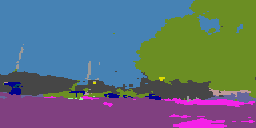
\includegraphics[width=20mm,height=10mm]{assets/fig3_tiny_probe.png}};
  \node[title, anchor=south] at ([yshift=1.8mm]probe.north) {Tiny probe};
  \node[smalltext, anchor=north] at ([yshift=-1.2mm]probe.south) {fixed engine};

  \node[card, circle, minimum size=13mm, fill=risk!8, draw=risk, line width=0.9pt]
    (entropy) at (57,25) {$s(x)$};
  \node[title, anchor=south] at ([yshift=2.0mm]entropy.north) {Visual risk};
  \node[smalltext, anchor=north] at ([yshift=-1.2mm]entropy.south) {mean entropy};

  \node[stage, anchor=west, minimum width=24mm, minimum height=21mm] (risks) at (67,25) {};
  \node[title, anchor=north] at ([yshift=-1.2mm]risks.north) {Candidate risk};
  \foreach \name/\col/\yy in {T/tiny/3.8,S/small/0.6,M/medium/-2.6,L/large/-5.8}{
    \draw[\col, line width=2.2pt, line cap=round]
      ([xshift=-9mm,yshift=\yy mm]risks.center) -- ([xshift=5mm,yshift=\yy mm]risks.center);
    \node[font=\fontsize{6.2}{7}\selectfont, anchor=west, text=ink]
      at ([xshift=7mm,yshift=\yy mm]risks.center) {$g_{\name}(s(x))$};
  }

  \node[stage, anchor=west, minimum width=22mm, minimum height=21mm] (costs) at (97,25) {};
  \node[title, anchor=north] at ([yshift=-1.2mm]costs.north) {Measured cost};
  \node[font=\sffamily\fontsize{6.2}{7}\selectfont, text=hardware] at ([yshift=3.2mm]costs.center)
    {$C_h(T)\quad C_h(S)$};
  \node[font=\sffamily\fontsize{6.2}{7}\selectfont, text=hardware] at ([yshift=-1.2mm]costs.center)
    {$C_h(M)\quad C_h(L)$};
  \draw[hardware, dashed, line width=0.7pt]
    ([xshift=-9mm,yshift=-6mm]costs.center) -- ([xshift=9mm,yshift=-6mm]costs.center)
    node[right, font=\sffamily\fontsize{6.2}{7}\selectfont, text=ink] {$B_h$};

  \node[diamond, draw=hardware, fill=panel, aspect=1.55, inner sep=1.2mm,
        font=\fontsize{6.3}{7.2}\selectfont\bfseries, align=center, text=ink]
    (filter) at (127,25) {budget\\feasible?};
  \node[smalltext, anchor=north] at ([yshift=-2.0mm]filter.south) {$C_h(\ell)\leq B_h$};

  \node[card, minimum width=13mm, minimum height=13mm, draw=medium, line width=1.2pt,
        fill=medium!8, font=\fontsize{7.2}{8}\selectfont\bfseries]
    (engine) at (141,25) {$\ell^*$};
  \node[title, anchor=south] at ([yshift=2.0mm]engine.north) {Static engine};

  \node[card, anchor=south west, inner sep=0.8mm] (output) at (151,19)
    {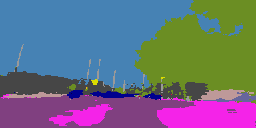
\includegraphics[width=20mm,height=10mm]{assets/fig3_selected_output.png}};
  \node[title, anchor=south] at ([yshift=1.8mm]output.north) {Segmentation};

  \draw[arr] (input.east) -- (probe.west);
  \draw[arr] (probe.east) -- (entropy.west);
  \draw[arr] (entropy.east) -- (risks.west);
  \draw[arr] (risks.north east) -- ++(2,6) -| (filter.north);
  \draw[arr] (costs.east) -- ([yshift=-3mm]filter.west);
  \draw[arr] (filter.east) -- (engine.west);
  \draw[arr] (engine.east) -- (output.west);

\end{tikzpicture}
\end{document}
